\documentclass[12pt, a4paper, twoside]{article}
\usepackage{hyperref}
\usepackage[utf8]{inputenc}
\usepackage[spanish]{babel}
\usepackage{xcolor}
\usepackage{csquotes}
\usepackage{graphicx}
\usepackage{float}
\usepackage{listings}
\usepackage[sorting=ydnt,bibstyle=reading,entryhead=true,natbib=true,citestyle=numeric]{biblatex}
\usepackage[a4paper,top=2cm,bottom=2cm,left=3cm,right=3cm,marginparwidth=1.75cm]{geometry}
\addbibresource{biblio.bib}

\lstdefinestyle{codeStyle}{
    backgroundcolor=\color{gray!10},
    commentstyle=\color{green!50!black},
    keywordstyle=\color{blue},
    numberstyle=\tiny\color{gray},
    stringstyle=\color{orange},
    basicstyle=\ttfamily\small,
    breaklines=true,
    frame=single,
    numbers=left,
    numbersep=8pt,
    tabsize=2,
    showstringspaces=false
}

%opening
\title{Laboratorio 2: IaC con Terraform y Cloud-Init sobre OpenStack}
\author{Guillermo Blazquez Ortega, \href{mailto:blazor@alumni.uv.es}{blazor@alumni.uv.es}} 
\date{\today{}}


\begin{document}
\maketitle

\begin{abstract}
	\begin{center}
		Uso de terraform como IaC para construir una infraestructura sobre OpenSatck y cloud-init para la
	 condifguracion y despliegue de una servicio sobre docker container.
	\end{center}
\end{abstract}

\tableofcontents
\clearpage

\section{Introduccion}

\begin{figure}[h!]
  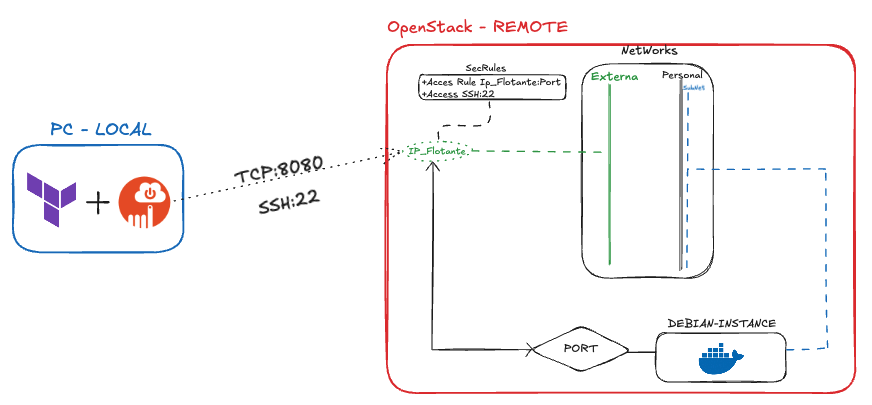
\includegraphics[width=\linewidth]{img/infra-img.png}
  \caption{Infraestructura Deseada}
  \label{fig:infra-basica}
\end{figure}
\lstinputlisting[style=codeStyle,caption={Código del Provider}]{code/providers.tf}


%Bibliografia Final
\clearpage
\nomention
\printbibliography[title={Bibliografia}]

\end{document}
